\documentclass[10pt,a4paper]{report}
\usepackage[utf8]{inputenc}
\usepackage[T2A]{fontenc}
\usepackage[utf8]{inputenc}
\usepackage[russian]{babel}
\usepackage{graphicx}
\usepackage{color}
\usepackage{subcaption}
\usepackage[export]{adjustbox}
\usepackage{scrextend}
\usepackage[inline]{enumitem}
\usepackage{xcolor}
\usepackage{mathtools}
\usepackage{cite}
\usepackage{comment}
\usepackage{multirow}

\title{Летняя практика}
\author{Полина Кадейшвили БПМИ2111}
\date{Июль 2022}

\begin{document}

\maketitle

\tableofcontents 
%\part{Часть первая}
\chapter{Кусочек текста из книги}
\section{Глава первая}
В начале июля, в чрезвычайно жаркое время, под вечер, один молодой человек вышел из своей каморки, которую нанимал от жильцов в С — м переулке, на улицу и медленно, как бы в нерешимости, отправился к К — ну мосту.


Он благополучно избегнул встречи с своею хозяйкой на лестнице. Каморка его приходилась под самою кровлей высокого пятиэтажного дома и походила более на шкаф, чем на квартиру. Квартирная же хозяйка его, у которой он нанимал эту каморку с обедом и прислугой, помещалась одною лестницей ниже, в отдельной квартире, и каждый раз, при выходе на улицу, ему непременно надо было проходить мимо хозяйкиной кухни, почти всегда настежь отворенной на лестницу. И каждый раз молодой человек, проходя мимо, чувствовал какое-то болезненное и трусливое ощущение, которого стыдился и от которого морщился.Он был должен кругом хозяйке и боялся с нею встретиться.


Не то чтоб он был так труслив и забит, совсем даже напротив; но с некоторого времени он был в раздражительном и напряженном состоянии, похожем на ипохондрию. Он до того углубился в себя и уединился от всех, что боялся даже всякой встречи, не только встречи с хозяйкой. Он был задавлен бедностью; но даже стесненное положение перестало в последнее время тяготить его. Насущными делами своими он совсем перестал и не хотел заниматься. Никакой хозяйки, в сущности, он не боялся, что бы та ни замышляла против него. Но останавливаться на лестнице, слушать всякий вздор про всю эту обыденную дребедень, до которой ему нет никакого дела, все эти приставания о платеже, угрозы, жалобы, и при этом самому изворачиваться, извиняться, лгать, — нет уж, лучше проскользнуть как-нибудь кошкой по лестнице и улизнуть, чтобы никто не видал.


Впрочем, на этот раз страх встречи с своею кредиторшей даже его самого поразил по выходе на улицу\cite{dostoyevsky2017crime}
\clearpage
\chapter{Сложные таблицы}
\section{Нейроны и медиаотры вегетативной нервной системы}

\begin{tabular}{ l | c | c }
\hline
  Нейроны & Локализация тел & Медиатор \\
  \hline
  \hline
  \multirow{2}{10em}{Парасимптатические преганглионарные} & 1.Ствол мозга & \multirow{2}{10em}{AX} \\
  & 2.Кересцовый отдел &\\
  \hline
  \multirow{2}{10em}{Cимптатические постганглионарные} & 1.Симпатический ствол & \multirow{2}{10em}{HA} \\
  & 2.Симпатические сплетения & \\
    \hline
\end{tabular} \\

\section{Вторая таблица (информация придумана и не соответвует действительнтсти)}
\begin{table}[h!]
    \begin{center}
    \caption{Информация о городах}
    \label{tab:table1}
    \begin{tabular}{l|c|c|r}
        \hline
        \textbf{город} & \textbf{Москва} & \textbf{Питер} & \textbf{Архангельск}\\
        \hline
        \hline
        \textbf{население} & \multicolumn{2}{c|}{652334} & 123243\\ 
        \hline
        \textbf{кол-во транспорты} & 10000 & 13124 & 213
    \end{tabular}
  \end{center}
\end{table}



\chapter{Вставка картинок}

\begin{figure}[t]
    \centering
    \begin{subfigure}{0.8\textwidth}
    \center{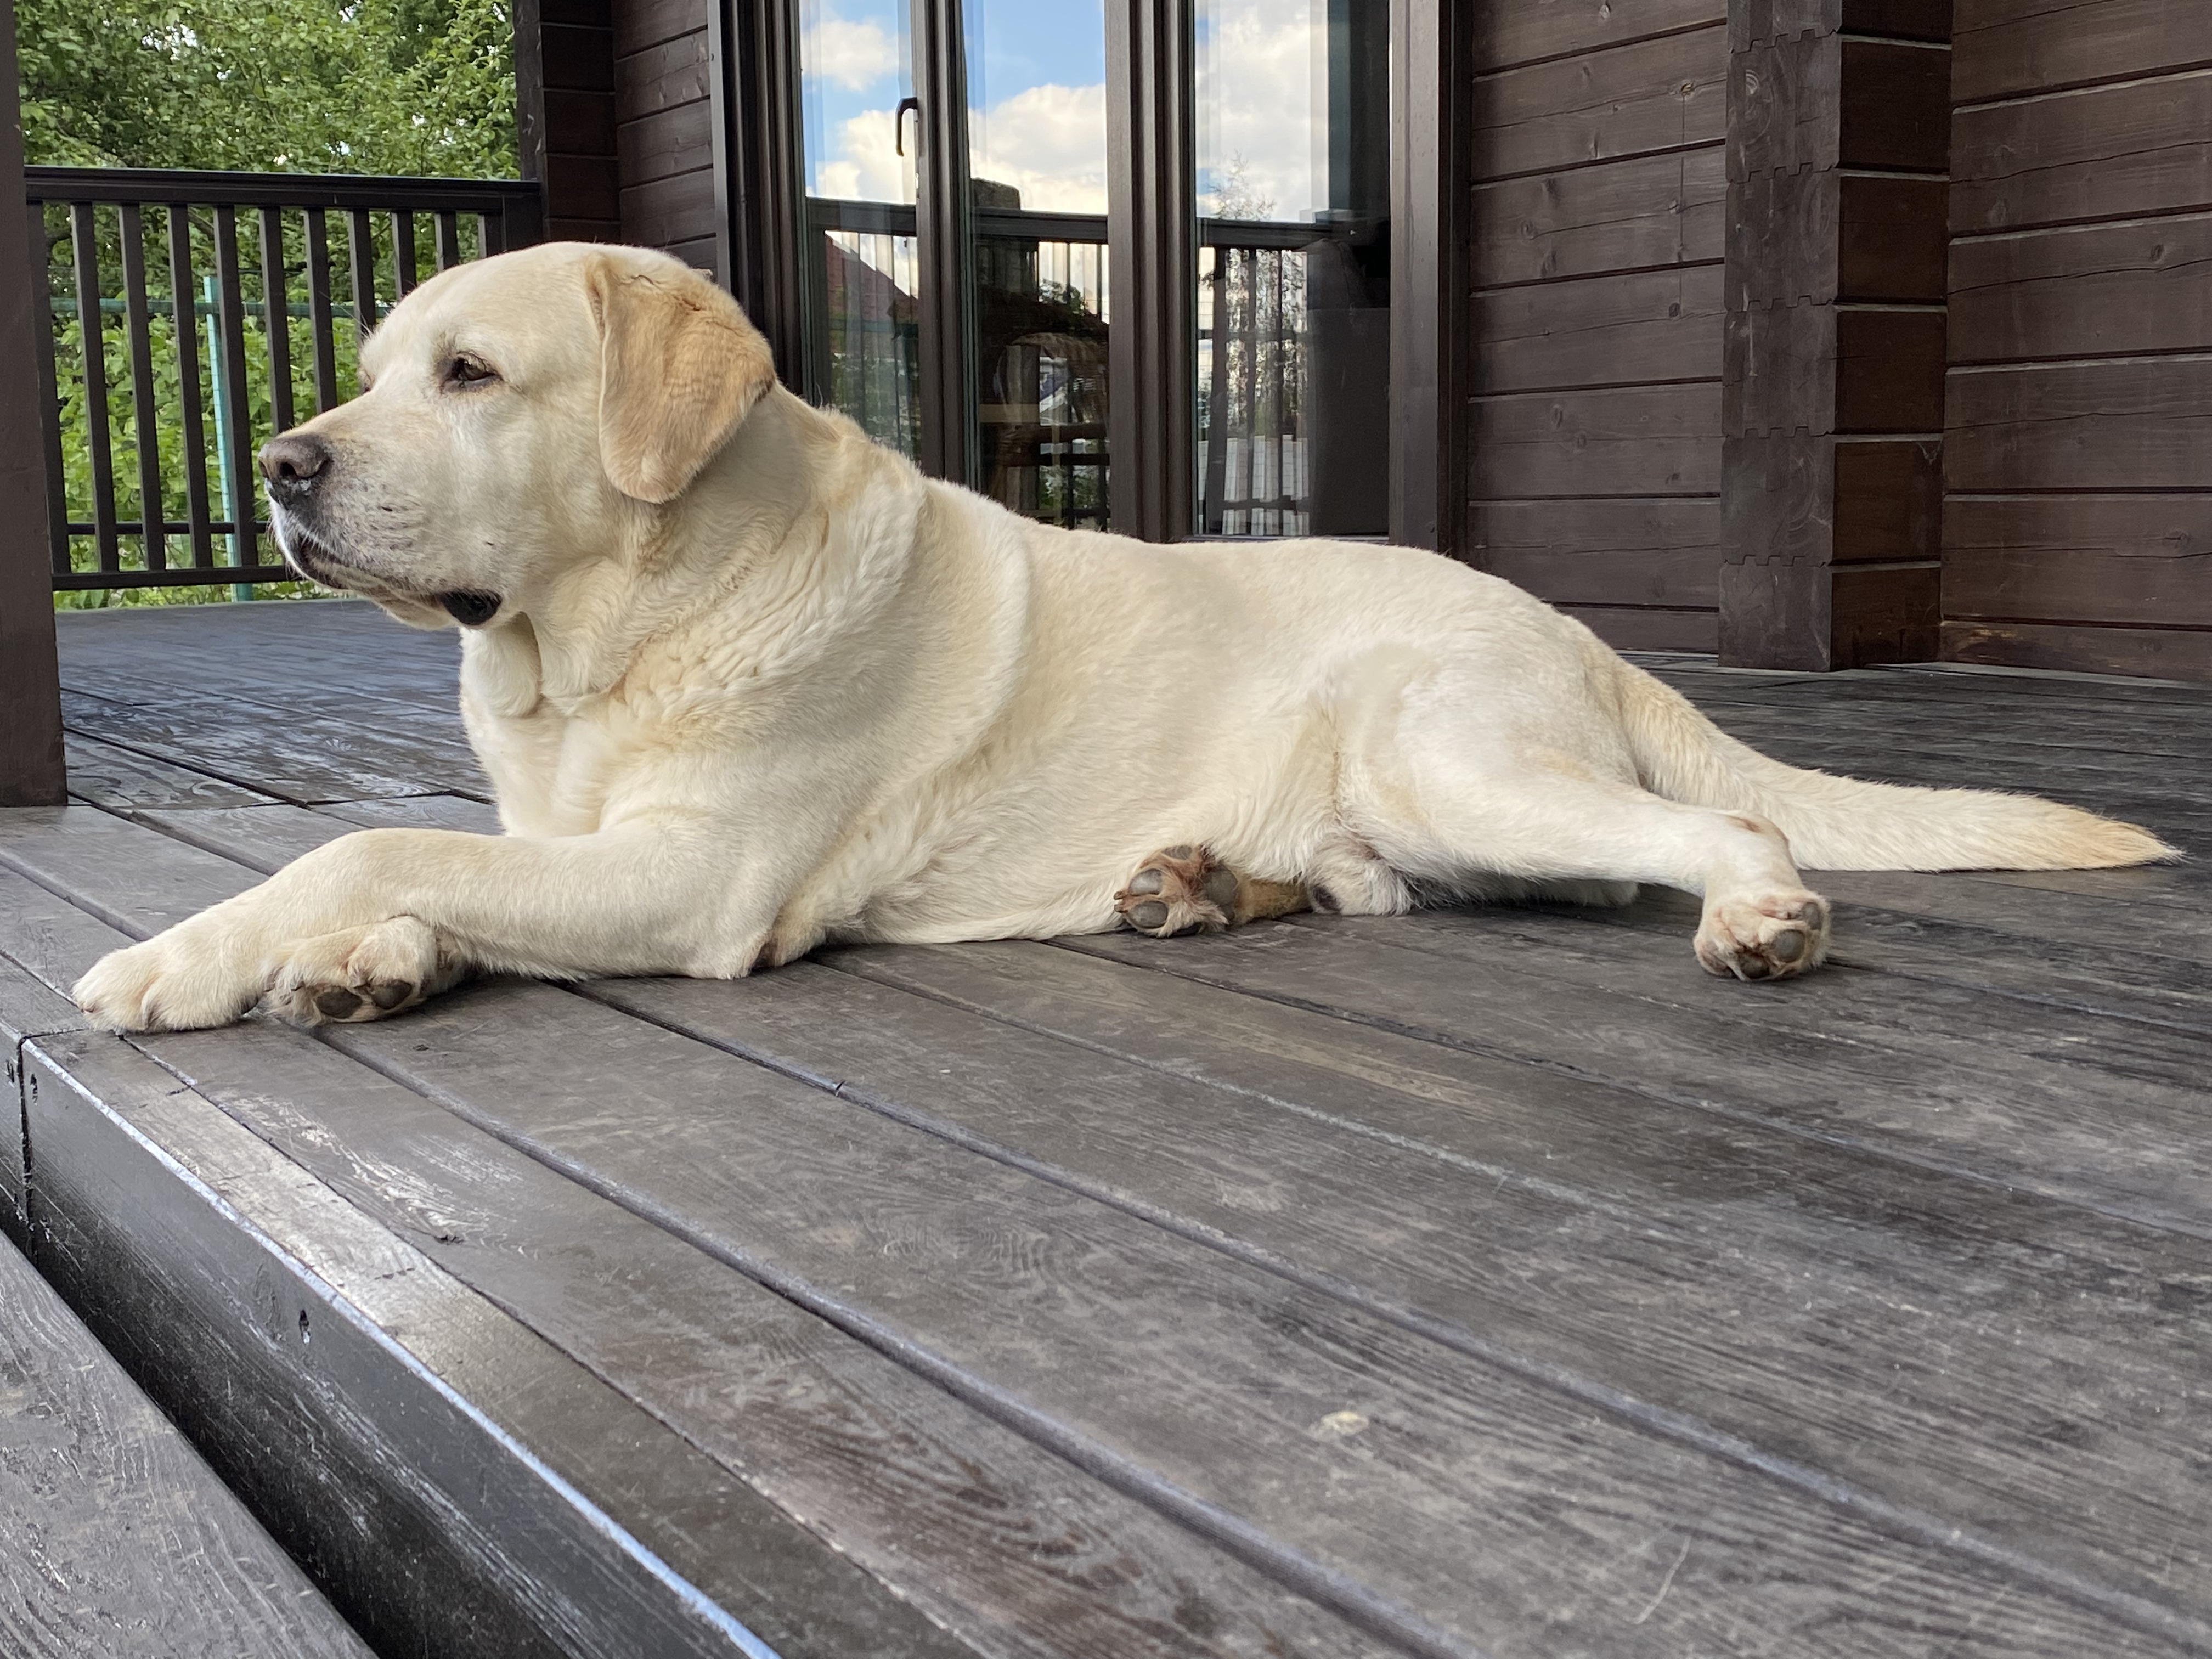
\includegraphics[width=0.6\textwidth]{images/IMG_2589.jpg}}
    \caption{Tired dog}
    \label{fig1}
    \end{subfigure}
    \begin{subfigure}{1\textwidth}
    \center{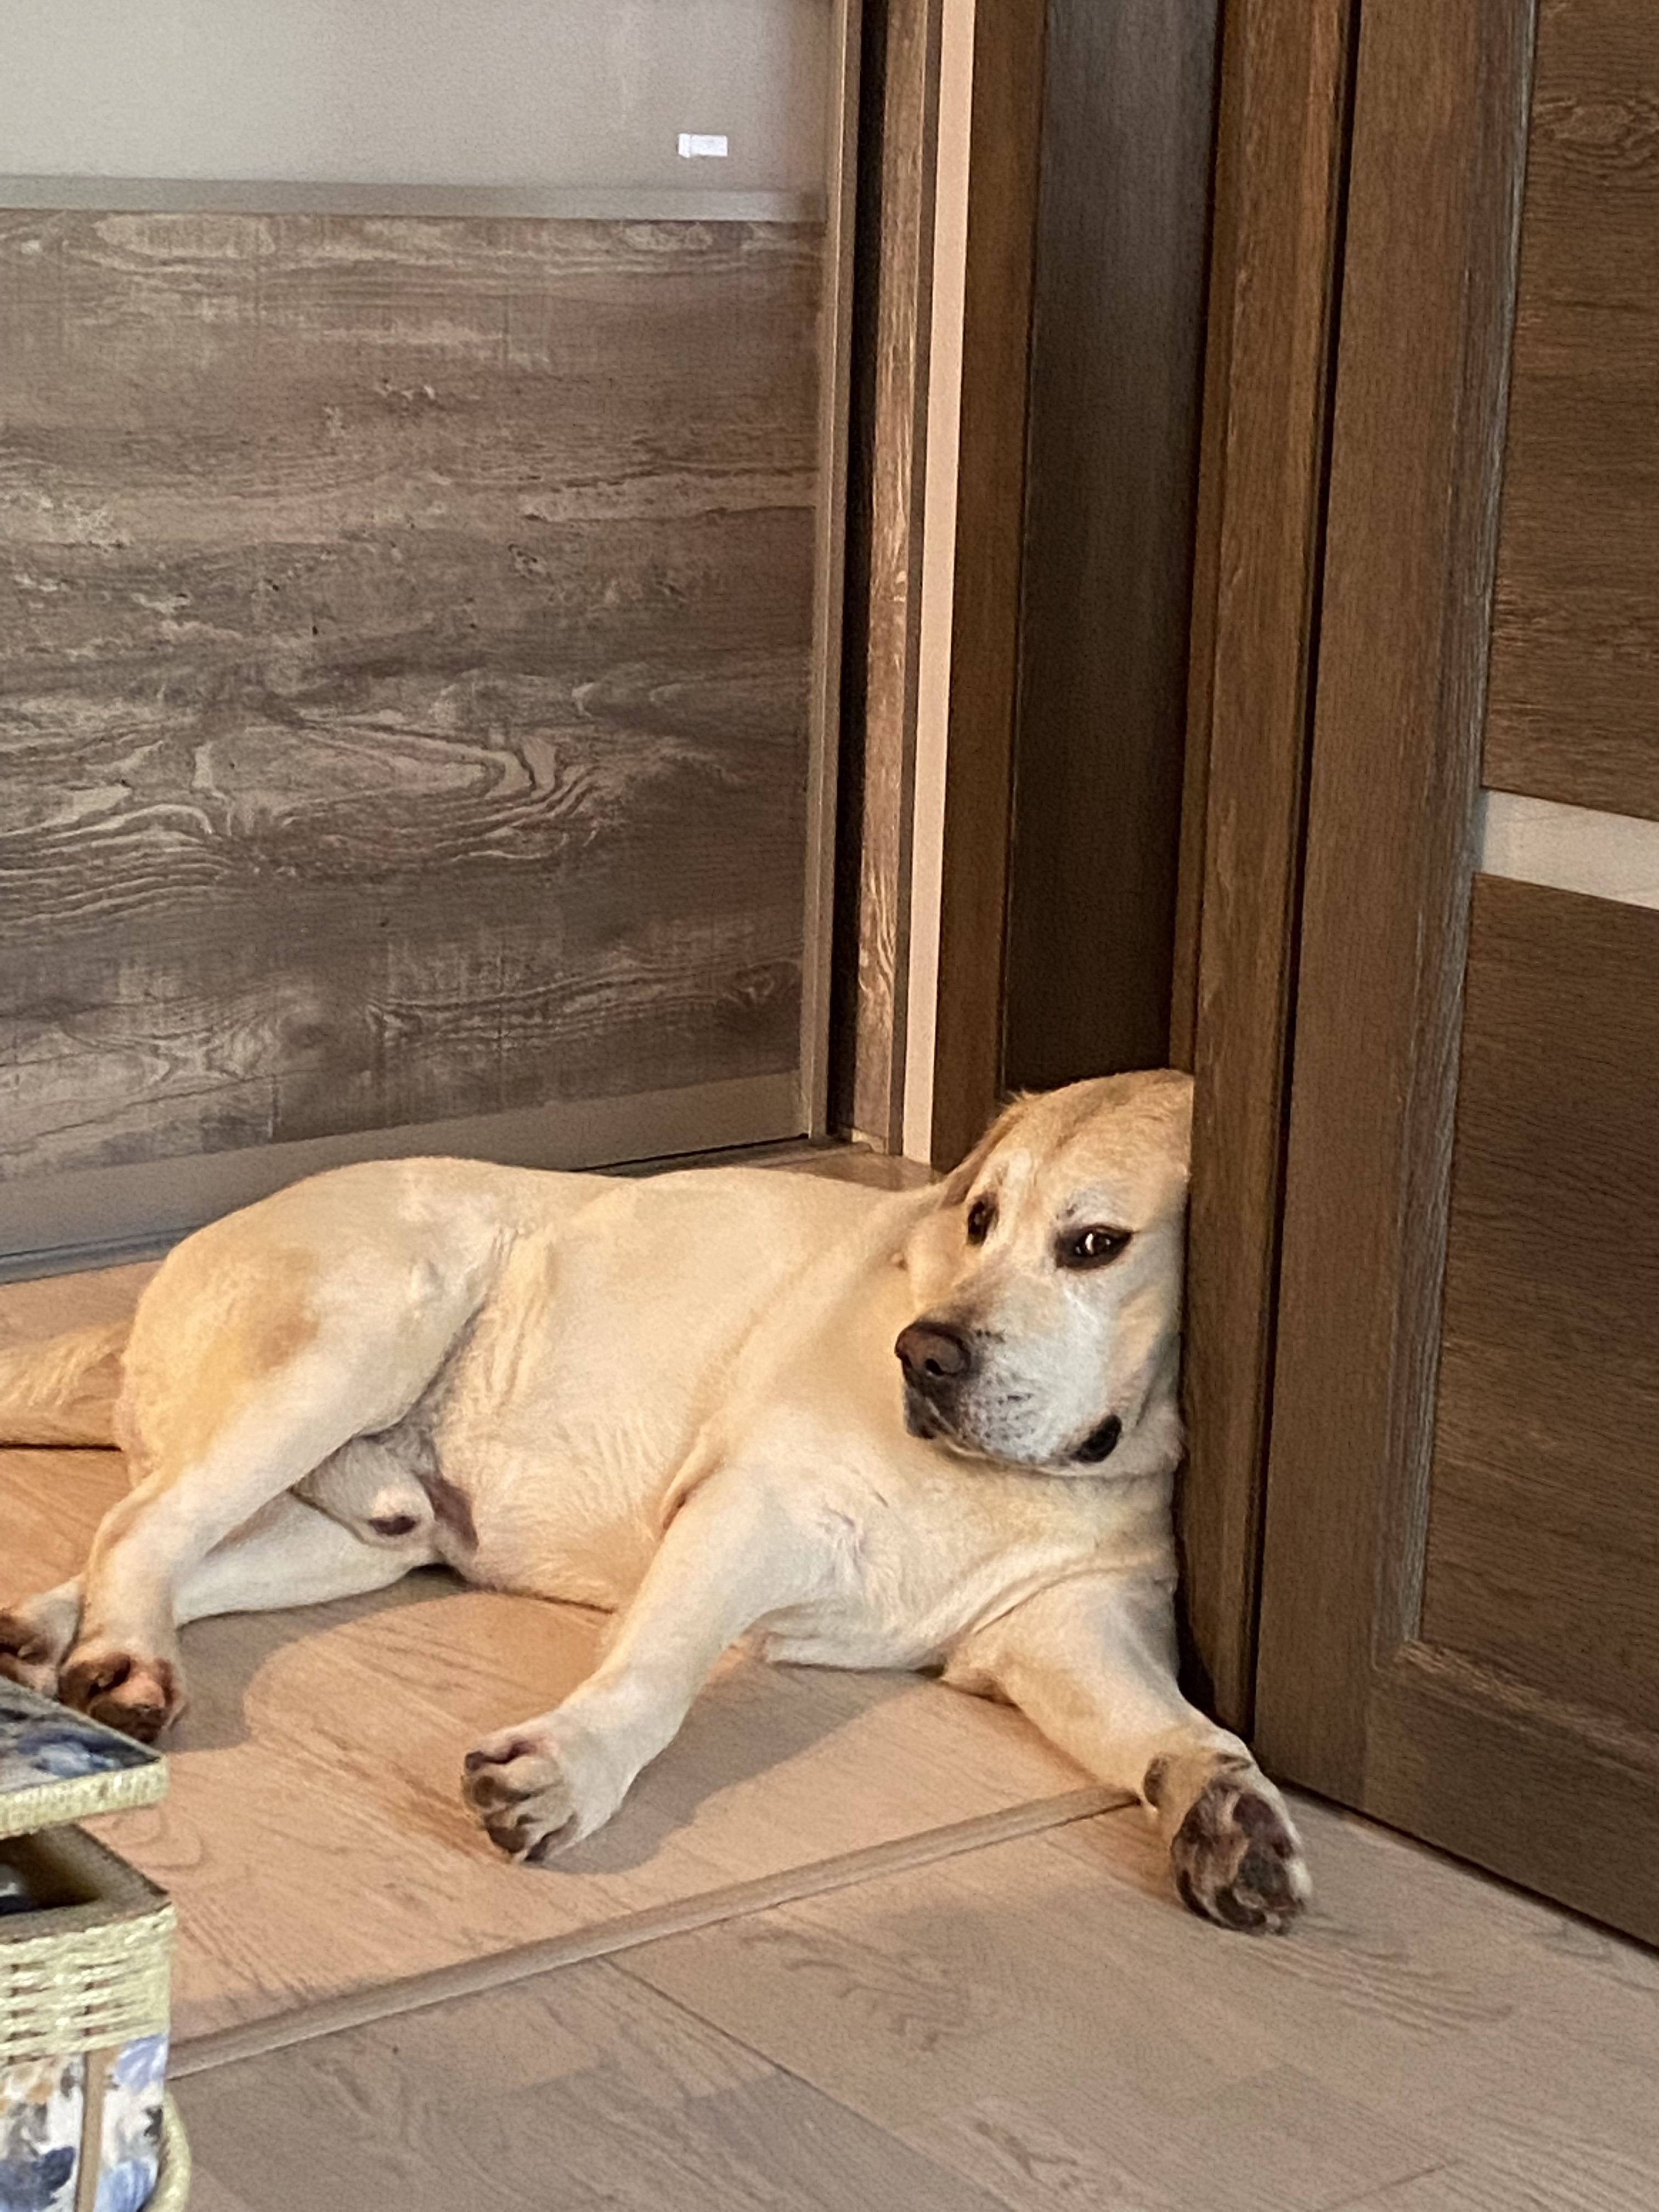
\includegraphics[width=0.6\textwidth]{images/IMG_2003.jpg}}
    \caption{Crazy dog}
    \label{fig2}
    \end{subfigure}
    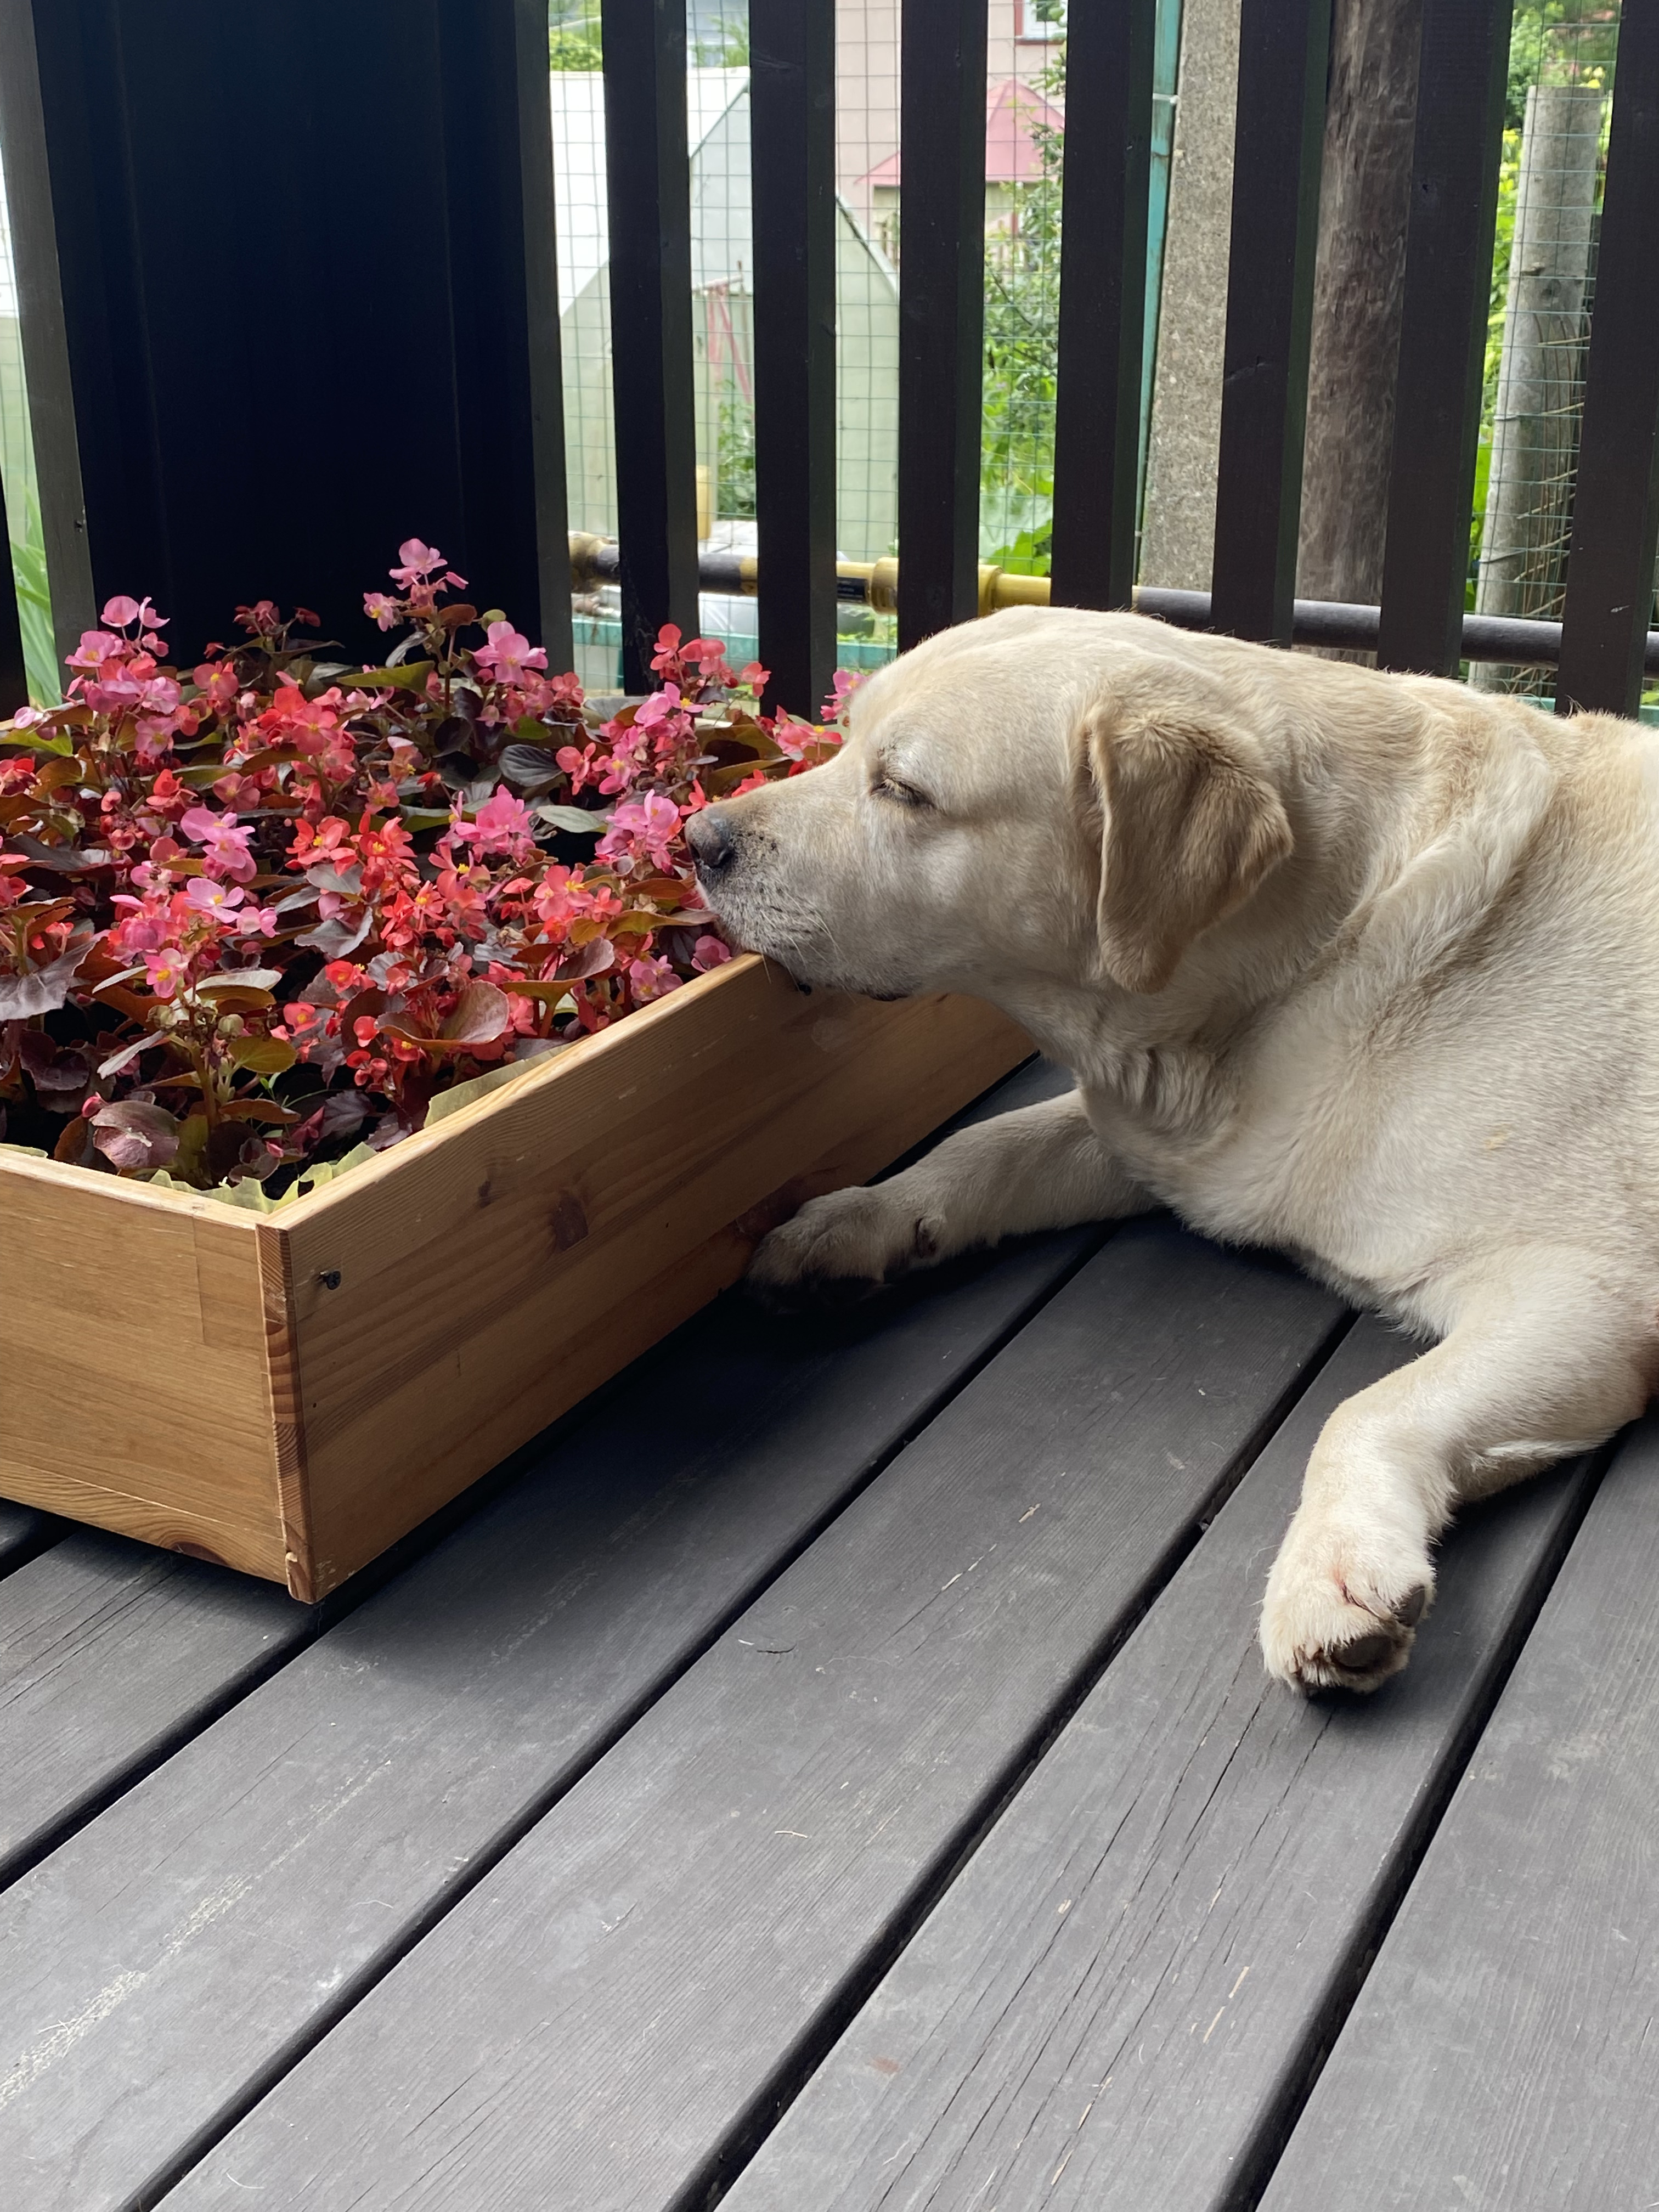
\includegraphics[height=0.6\textwidth]{images/IMG_8476.jpg}
    \includegraphics[height=0.6\textwidth]{images/IMG_8352.jpg}
    \caption{happy dog}
    \label{fig3}
\end{figure}
\Large
Далее, чтобы поработать с изображениями, я выбрала  несколько фото своей собаки и сделала из них некую композицию, результат можно уивдеть на следующей странице: \ref{fig1}, \ref{fig2} и \ref{fig3}
\normalsize

\chapter{Листы}
\section{Неупорядоченный список стандартных покупок}
\begin{itemize}
	\item молоко 
	\item хлеб
	\item кефир
    \item соль
\end{itemize}

\noindent\rule{\textwidth}{1pt}

\section{Упорядоченный список глав}
\begin{enumerate}  
	\item Первая глава
	\item Вротая глава
	\item Третья глава
\end{enumerate}

\noindent\rule{\textwidth}{1pt}

\section{Вложенный список - виды блюд}
\begin{enumerate}
	\item Основное блюдо
	\begin{enumerate}
		\item Горячее
        \begin{enumerate}
            \item Суп
            \item Основное блюдо
        \end{enumerate}
		\item Холодное
		\begin{enumerate}
		\item Закуски
		\item Салаты
	    \begin{enumerate}
		\item Вегетерианские салаты
        \item Салаты с мясом

	\end{enumerate}
	\end{enumerate}
	\end{enumerate}
		\item Закуски
		\item Десерты 
        \item Напитки
\end{enumerate}
\clearpage

\chapter{Математические формулы}
\section{Универсальные тригонометрические замены}
$t = \tan\frac{x}{2}$\\
$\sin(x) = \frac{2\tan(\frac{x}{2})}{1 + \tan^2(\frac{x}{2})} = \frac{2t}{1 + t^2}$\\
$\cos(x) = \frac{1 - \tan^2(\frac{x}{2})}{1 + \tan(\frac{x}{2})} = \frac{1 - t^2}{1 + t^2}$

\section{Формула из доказательства корректонсти ряда Тейлора}
$|\ln{(1 + x)} - \sum_{n=1}^{m}\frac{(-1)^{n-1}x^n}{n}| = \int_{0}^{x} (x-t)^m \cdot \frac{1}{(1+t)^{m+1}} \mathrm{d}t$

\section{Пример задания функции}
$ f(n) =
  \begin{cases}
    \frac{2xy}{x^2 + y^2}       & \quad \text{if } (x, y) \mathrel{\mathtt{!=}}\ (0, 0)\\
    0  & \quad \text{if } (x, y) = (0, 0)
  \end{cases}
$
\section{Предел функции по Коши}
$\forall \epsilon > 0 \quad \exists \delta>0: \forall x: {0 < |x-a| < \delta} \Rightarrow {|f(x) - A|< \epsilon}$
\clearpage

\chapter{Библиография и цитирование}


Comparison of data representations is a complex multi-aspect problem that has not enjoyed a complete solution yet. We propose a method for comparing two data representations. We introduce the Representation Topology Divergence (RTD), measuring the dissimilarity in multi-scale topology between two point clouds of equal size with a one-to-one correspondence between points. The data point clouds are allowed to lie in different ambient spaces. The RTD is one of the few TDA-based practical methods applicable to real machine learning datasets. Experiments show that the proposed RTD agrees with the intuitive assessment of data representation similarity and is sensitive to its topological structure. We apply RTD to gain insights on neural networks representations in computer vision and NLP domains for various problems: training dynamics analysis, data distribution shift, transfer learning, ensemble learning, disentanglement assessment.\cite{barannikov2021representation}


Ну и вот вам умный термин: интерполяция\footnote{Интерполяцией называют такую разновидность аппроксимации, при которой кривая построенной функции проходит точно через имеющиеся точки данных. В этой статье изучены формулы интерполяции Лагранжа и Ньютона в задаче интерполяции функции.}
\bibliographystyle{plain}
\bibliography{bibliography.bib}
\begin{comment}
    это комментарий, который не будет показан
    можно писать в несколько строк
\end{comment}
\end{document}
